\PassOptionsToPackage{xetex}{xcolor}
\PassOptionsToPackage{xetex}{graphicx}
\documentclass[a4paper,landscape,headrule,footrule,xetex]{foils}

%%
%%%  Macros
%%%
\newcommand{\logo}{~}
\MyLogo{HG8011 (2019)}
\newcommand{\Story}{\SHA{HOUN}{The Hound of the Baskervilles}}

\newcommand{\header}[3]{%
\title{\vspace*{-2ex} \large Detecting Meaning with Sherlock Holmes\thanks{Creative Commons Attribution License: you are free to share and adapt as long as you give appropriate credit and add no additional restrictions: 
\protect\url{https://creativecommons.org/licenses/by/4.0/}.}
%\footnotemark
\\[2ex] \Large  \emp{#2} \\ \emp{#3}}
\author{\blu{Francis Bond}   \\ 
\normalsize  \textbf{Division of Linguistics and Multilingual Studies}\\
\normalsize  \url{http://www3.ntu.edu.sg/home/fcbond/}\\
\normalsize  \texttt{bond@ieee.org}}
 \date{Location: LT25}
 \renewcommand{\logo}{#2}
 \hypersetup{
   pdfinfo={
     Author={Francis Bond},
     Title={#2},
     Subject={HG8011: Detecting Meaning with Sherlock Holmes},
     Keywords={Semantics, Pragmatics, Meaning},
     License={CC BY 4.0}
   }
 %  pdfcopyright={Copyright © Francis Bond. Creative Commons 4.0 Attribution License.}
 %  pdflicenseurl={http://creativecommons.org/licenses/by/4.0/}
 }
}
%%
%% Multilingual Stuff
%%
\usepackage[a4paper,landscape,margin=25mm]{geometry}

\usepackage{fontenc}
\usepackage{polyglossia}
\setmainlanguage{english}
\setmainfont{TeX Gyre Pagella}
\usepackage{xeCJK}
\setCJKmainfont{Noto Sans CJK SC}
\setCJKsansfont{Noto Sans CJK SC}
\setCJKmonofont{Noto Sans CJK SC}
%\setCJKttfont{Noto Sans CJK SC}
%\setCJKmainfont{WenQuanYi Micro Hei}
%\clearpage
%\setCJKmainfont{AR PL SungtiL GB}

\usepackage[xetex]{xcolor}
\usepackage[xetex]{graphicx}
\newcommand{\blu}[1]{\textcolor{blue}{#1}}
\newcommand{\grn}[1]{\textcolor{green}{#1}}
\newcommand{\hide}[1]{\textcolor{white}{#1}}
\newcommand{\emp}[1]{\textcolor{red}{#1}}
\newcommand{\txx}[1]{\textbf{\textcolor{blue}{#1}}}
\newcommand{\lex}[1]{\textbf{\mtcitestyle{#1}}}

\usepackage{pifont}
\renewcommand{\labelitemi}{\textcolor{violet}{\ding{227}}}
\renewcommand{\labelitemii}{\textcolor{purple}{\ding{226}}}

\newcommand{\subhead}[1]{\noindent\textbf{#1}\\[5mm]}

\newcommand{\Bad}{\emp{\raisebox{0.15ex}{\ensuremath{\mathbf{\otimes}}}}}
\newcommand{\bad}{*}

\newcommand{\com}[1]{\hfill \textnormal{(\emp{#1})}}%
\newcommand{\cxm}[1]{\hfill \textnormal{(\txx{#1})}}%
\newcommand{\cmm}[1]{\hfill \textnormal{(#1)}}%
\usepackage{amssymb}
\usepackage{relsize,xspace}
\newcommand{\into}{\ensuremath{\rightarrow}\xspace}
\newcommand{\ent}{\ensuremath{\Rightarrow}\xspace}
\newcommand{\nent}{\ensuremath{\not\Rightarrow}\xspace}
\newcommand{\tot}{\ensuremath{\leftrightarrow}\xspace}
\usepackage{url}
\usepackage[hidelinks]{hyperref}
\hypersetup{
     colorlinks,
     linkcolor={blue!50!black},
     citecolor={red!50!black},
     urlcolor={blue!80!black}
}
%\usepackage{hyperxmp}
\newcommand{\lurl}[1]{\MyLogo{\url{#1}}}

\usepackage{mygb4e}
\let\eachwordone=\itshape
\newcommand{\lx}[1]{\textbf{\textit{#1}}}
\newcommand{\ix}{\ex\it}

\newcommand{\cen}[2]{\multicolumn{#1}{c}{#2}}
%\usepackage{times}
%\usepackage{nttfoilhead}
\newcommand{\myslide}[1]{%
\foilhead[-25mm]{\raisebox{12mm}[0mm]{\emp{#1}}}%
\leftheader{}%
\MyLogo{\logo}}

\newcommand{\mytask}[1]{%
\foilhead[-25mm]{\raisebox{12mm}[0mm]{\emp{#1}}}
\leftheader{🔍 Hi}%
\MyLogo{\logo}}

\newcommand{\myslider}[1]{\rotatefoilhead[-25mm]{\raisebox{12mm}[0mm]{\emp{#1}}}}
%\newcommand{\myslider}[1]{\rotatefoilhead{\raisebox{-8mm}{\emp{#1}}}}

\newcommand{\section}[1]{\myslide{}{\begin{center}\Huge \emp{#1}\end{center}}}

\usepackage{tcolorbox}
% \newcommand{\task}{\marginpar{\raisebox{-1ex}{\large
%       \tcbox[colframe=red,colback=white,arc=3pt]{\textbf{?}}}}}
% \newcommand{\task}{\marginpar{\raisebox{-1ex}{
%       \hspace{-0.5em}\tcbox[colframe=red,colback=white,arc=3pt]{%
%         
\includegraphics[width=1.5em]{pics/detective}}}}}
\newcommand{\task}{\marginpar{\raisebox{-2ex}{
      \hspace{-0.5em}\reflectbox{
\includegraphics[width=2em]{pics/detective}}}}}

\usepackage[lyons,j,e,k]{mtg2e}
\renewcommand{\mtcitestyle}[1]{\textcolor{teal}{\textsl{#1}}}
%\renewcommand{\mtcitestyle}[1]{\textsl{#1}}
\newcommand{\chn}{\mtciteform}
\newcommand{\cmn}{\mtciteform}
\newcommand{\iz}[1]{\textup{\texttt{\textcolor{blue}{\textbf{#1}}}}}
\newcommand{\con}[1]{\textsc{#1}}
\newcommand{\gm}{\textsc}
\newcommand{\cmp}[1]{{[\textsc{#1}]}}
\newcommand{\sr}[1]{\ensuremath{\langle}#1\ensuremath{\rangle}}
\usepackage[normalem]{ulem}
\newcommand{\ul}{\uline}
\newcommand{\ull}{\uuline}
\newcommand{\wl}{\uwave}
\newcommand{\vs}{\ensuremath{\Leftrightarrow}~}
%%%
%%% Bibliography
%%%
\usepackage{natbib}
%\usepackage{url}
\usepackage{bibentry}


%%% From Tim
\newcommand{\WMngram}[1][]{$n$-gram#1\xspace}
\newcommand{\infers}{$\rightarrow$\xspace}



\usepackage{rtrees,qtree}
\renewcommand{\lf}[1]{\br{#1}{}}
\usepackage{avm}
%\avmoptions{topleft,center}
\newcommand{\ft}[1]{\textsc{#1}}
%\newcommand{\val}[1]{\textit{#1}}
\newcommand{\typ}[1]{\textit{#1}}
\avmfont{\sc}
%\avmvalfont{\sc}
\renewcommand{\avmtreefont}{\sc}
\avmsortfont{\it}


%%% From CSLI book
\newcommand{\mc}{\multicolumn}
\newcommand{\HD}{\textbf{H}\xspace}
\newcommand{\el}{\< \>}
\makeatother
\long\def\smalltree#1{\leavevmode{\def\\{\cr\noalign{\vskip12pt}}%
\def\mc##1##2{\multispan{##1}{\hfil##2\hfil}}%
\tabskip=1em%
\hbox{\vtop{\halign{&\hfil##\hfil\cr
#1\crcr}}}}}
\makeatletter

\newcommand{\sh}[1]{\lowercase{\href{https://fcbond.github.io/sh-canon/#1.html}}{#1}}
\newcommand{\SHA}[2]{\lowercase{\href{https://fcbond.github.io/sh-canon/#1.html}}{\textit{#2}}}

\newcommand{\tra}[1]{\textcolor{olive}{\textsf{#1}}}
\usepackage{multicol}
\usepackage{booktabs,subscript}
\newcommand{\DF}[1]{\parbox{.6\textwidth}{#1}}
\begin{document}
\makexeCJKinactive
\renewcommand{\avmvalfont}{\it}
\header{~}{Screening Sherlock Holmes}{\normalsize based on slides by Brian Bergen-Aurand}
%Film Studies and Literature
\maketitle


\myslide{Overview}
\MyLogo{Film Studies and Literature}
\begin{itemize}
\item How (Screen) Language
  Conveys Meaning
  \begin{center}
  — Christian Metz Screens Sherlock Holmes  —
      \end{center}
\item 
Sherlock Holmes Baffled — Signs and
Interpretations
\item 
The Language of Screen Theory
\item Film Language: A Semiotics of the Cinema
\item The Adventure of the Speckled Band 1 \& 2
\end{itemize}
\myslide{Sherlock Holmes Baffled}

\href{https://www.youtube.com/watch?v=HYN4QzX9-EM}{Sherlock Holmes Baffled}

\begin{itemize} 
\item directed by Arthur Marvin in 1905 (music added)
\end{itemize}

\myslide{Sherlock Holmes Baffled} 

\begin{tabular}{cc}
Signs & Interpretations \\
  \begin{minipage}{0.45\linewidth}
    \begin{itemize}
    \item Holmes alone
    \item Smoking a cigar
    \item Holmes unkempt
\item Holmes draws and fires a gun
\item Holmes is “baffled”
\item A crime against Holmes
\item Holmes in the \textit{domestic}
sphere
    \end{itemize}
  \end{minipage}
  &
  \begin{minipage}{0.45\linewidth}
  \end{minipage}
\end{tabular}
\newpage
\begin{itemize}
\item Films start in 1895 
  \begin{itemize}
  \item  standard viewing position (front)
  \item  charge admissions
  \end{itemize}
\item Early films had a fixed camera
  \begin{itemize}
  \item So drawing rooms scenes were common
  \end{itemize}
\item What does Holmes look like \task
%%% Cap, pipe, magnifying glass, cape
  \begin{itemize}
  \item What is different in \textit{Sherlock Holmes baffled}?
  \item What is in the center?
  \item What is he wearing?
  \item What is the big difference in the narrative?
    \begin{itemize}
    \item No Watson!
    \end{itemize}
  \end{itemize}
  
\myslide{Cinematic Signs / Cinematic Language}
\begin{itemize}
\item Themes and ideas
\item Film and the other arts
\item Realism, anti-realism, and \textit{mise-en-scène}
\\ ``telling a story through the cinematography, stage design and storyboarding''
\item Composition and the image
\item Sound
\end{itemize}

\myslide{The Language of Screen Theory}
\begin{itemize}
\item What is cinema?
  \begin{itemize}
  \item Cinema is a language in the sense of a
semiotic system.
\item Semiotics (semiology) is the science of
signs and of the codes used to understand
them
\end{itemize}
\item How do we understand it?
  \begin{itemize}
  \item The system of every film is constructed on
the basis of codes that a filmmaker either
adopts, transforms, or works against.

\end{itemize}
\end{itemize}

\myslide{A Semiotics of the Cinema}
\MyLogo{Christian Metz}
\begin{quotation}
  
\end{quotation}
“Everything is present in film: hence the
obviousness of film, and hence also its opacity.
The clarification of present by absent units
occurs much less than in verbal language. The
relationships \textit{in praesentia} are so rich that
they render the strict organization of \textit{in
absentia} relationships superfluous and
difficult. A film is difficult to explain because it
is easy to understand. The image impresses
itself on us, blocking everything that is not
itself.”
\end{itemize}
Christian Metz (2015). \textit{Impersonal Enunciation, or the Place of Film} p.11, Columbia University Press

% Christian Metz:
% A Semiotics of the Cinema
% Inspector Bourrel, from the French TV show
% Les cinq dernières minutes (1958-92) in
% Impersonal Enunciation (2016).
% Story and Discourse
% Diegetic and Extra-Diegetic Narration
% When the detective speaks about the case
% to characters / to the audience
\myslide{Reception: A Semiotics of Holmes}
\MyLogo{Two ways of looking at films (or anything)}
\begin{itemize}
\item Analyze the stories as detective fiction
  \begin{itemize}
  \item Structure, logic, and the nature of detection
    \begin{itemize}
    \item Genre, technique, narrative
      \begin{itemize}
      \item Story \& Discourse %(Enunciation)
      \end{itemize}
    \item Similar to the books, but with a different vocabulary
      \begin{itemize}
      \item easy to show
      \item hard to explain
      \item limited in space and time
      \end{itemize}
    \end{itemize}
  \end{itemize}
\item Analyze the stories as cultural representation
  \begin{itemize}
  \item Social and historical implications and
    resonances
    \begin{itemize}
    \item Institutional structures and relationships
      \begin{itemize}
      \item Race, Class, Gender, Sexuality, Technology, Law, \ldots
      \end{itemize}
    \end{itemize}
  \end{itemize}
\end{itemize}
\myslide{The Speckled Band}
\begin{itemize}
\item \href{https://www.youtube.com/watch?v=1pGT51t5xNE}{The Case of
    the Speckled
    Band (1/2)} (12min)
\item \href{https://www.youtube.com/watch?v=L83Ugq8o3i8}{The Case of
    the  Speckled
    Band (1/2)} (12min)
\item \textit{Sherlock Holmes and Doctor Watson} is a television
  series created by Sheldon Reynolds in 1979
\item  It starred Geoffrey Whitehead, Donald Pickering and Patrick
  Newell in the title roles of Sherlock Holmes, Doctor Watson and
  Inspector Lestrade respectively.
\item It was a joint Polish-English production with 24 episodes

\item How is the story different?
\item Why doesn’t Holmes kill the snake?
\item Nice use of music to build suspense, \dots{}
\end{itemize}



% %%% Five major areas
% \item Cinematic Language
%  \begin{itemize}
%   \item Themes and Ideas
%   \item Film and other arts
%   \item Realism, anti-realism and \textit{mise-en-scène}
%   \item Composition and the image
%   \item Sound
%   \end{itemize}
% \item The language of Screen Theory  %%% slides
%   \begin{itemize}
%   \item What is cinema?
%   \item How do we understand it?
%   \end{itemize}
% \item Film works through five mediums  
%   \begin{itemize}
%   \item Image
%   \item Dialogue
%   \item Print
%   \item Music
%   \item Ambient sound and noise
%   \end{itemize}
% \item Diegetic (on-screen) and Extra-diegetic (off-screen)
% \end{itemize}

% \include{schedule}

\myslide{Speckled Band}
\begin{itemize}
\item Analyze the stories as detective fiction
  \begin{itemize}
  \item A rethinking of the detective in general, of Holmes
in particular
\item The detective in relation to the villain, Holmes in
relation to the Count
\end{itemize}
\item Analyze the stories as cultural representation
  \begin{itemize}
  \item Women in a society in which they cannot own
property \\ (the original story)
\item Women in a society in which they can own
property \\ (the TV story)
\end{itemize}

% \begin{itemize}
% \item Until 1882 (in England) women could not own property and were legally treated
%   the same as their guardian (father or husband)
% \item 
% \end{itemize}

\end{itemize}

\myslide{Screen Language — Signs}
\MyLogo{Repetition, Difference, and Ambiguity}

\begin{itemize}
\item The Adventure of the Speckled Band
\item “Miss Stoner, you have not. You are screening your
stepfather.”
\item 
  \begin{itemize}
  \item Count: Mr. Holmes do you ever hunt?
  \item Holmes: In a manner of speaking, Count.
  \item Count: Yes. Of course.
  \end{itemize}
\item Holmes: “I suppose we’ll have to think of the case
of the speckled band as only partially successful.”
\end{itemize}

\myslide{Sherlock Holmes in the 22nd Century}

An animated television series from 1999--2001 in which Sherlock Holmes
is brought back to life in the 22nd century to deal with a Moriarty
clone. The series was nominated for a Daytime Emmy for Special Class
Animated Program.


\hspace{-2.5cm}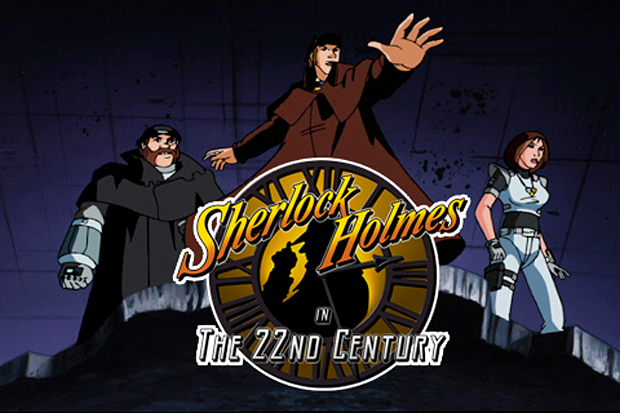
\includegraphics[height=0.6\textheight]{pics/Sherlock-Holmes-in-the-22nd-Century.jpg}}
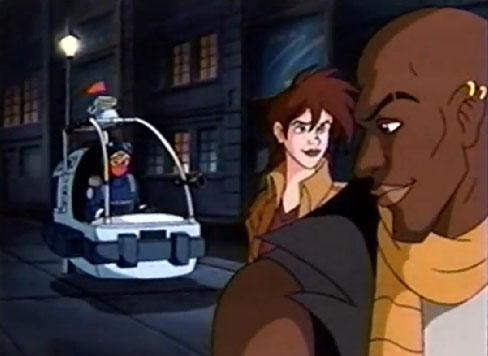
\includegraphics[height=0.6\textheight]{pics/22ndirregulars.JPG}}


Watch: \href{https://www.youtube.com/watch?v=d9Eiy5FvYO0}{The Adventure of
  the Dancing Men} (22 min)

\myslide{A more diverse cast}

\begin{itemize}
\item Inspector Beth Lestrade of New Scotland Yard 
\item The French rogue geneticist Martin Fenwick
\item A clone of Professor James Moriarty
\item A rejuvenated Sherlock Holmes (he had been preserved in honey)
\item A   droid Watson
\item The new Baker Street Irregulars
  \begin{itemize}
  \item football player Wiggins
  \item the Cockney Deidre
  \item paraplegic Tennyson
  \end{itemize}
\end{itemize}


\myslide{Compare / Contrast}
\begin{center}
  \begin{tabular}{cc}
    Readership & Viewership \\
    The reader’s surrogate & The viewers’ surrogates \\
    Holmes’s methodology & Holmes’s methodology\\
    Detection & Detection \\
    Making sense of things & Making sense of things
  \end{tabular}

  \begin{itemize}
  \item \txx{Audience surrogate} A focus character (or characters) who
    voices or experiences the thoughts, reactions and emotions which
    the writer desires the reader to have. Usually the point-of-view
    character, usually observing a scene or being acted upon.
    \begin{itemize}
    \item  Who is this in the Sherlock Holmes stories? \task
    \item Who is this in \textit{Sherlock Holmes in the 22nd Century}? \task
    \end{itemize}
  \end{itemize}

\end{center}
% In print (since 1887)
% On film (since 1900)
% On television (since ~1951)
% In video games (since 1984)
% On the internet (since 2004)Gaming Holmes
% Readership, Viewership,
% Playership
% http://www.sherlockian-sherlock.com/free-full-online-
% games.phpGaming Holmes
% The player’s surrogate
% Holmes’s methodology
% Detection
% Making sense of thingsFrom Screening Holmes
% to Translating Holmes
% Screening Holmes  Essay rather than
% adaptation.
% Screening Holmes involves a site of contact
% filled with repetition, difference, and
% ambiguity.
% Screening Holmes invites us to revisit all
% the texts and contexts involved in this
% contact zone.
% Sherlock Holmes in Translation
% Thank you!
\myslide{Screening Sherlock Holmes}
\begin{itemize}
\item In print (since 1887)
\item On film (since 1900)
\item On television (since ~1951)
\item In video games (since 1984)
\item On the internet (since 2004)
\end{itemize}



\myslide{Adaptions: Films}

\begin{itemize}
\item Guinness World Records lists Holmes as the "most portrayed movie
  character": more than 70 actors in over 200 films.
\item The first screen appearance was in the 30-second 1900 Mutoscope film: \textit{Sherlock Holmes Baffled}
\item New films appeared almost every year since then 
\item Basil Rathbone appeared in 14 films, starting with \sh{HOUN} in 1939
\item Robert Downey, Jr. (2009, 2011)
\item Ian McKellen (2015) \textit{Mr. Holmes}
\item Henry Cavill (2020) \textit{Enola Holmes}
\end{itemize}

\myslide{Adaptions: TV}
\begin{itemize}
\item Jeremy Brett appeared in \textit{The Adventures of Sherlock Holmes}
  \begin{itemize}
  \item Granada Television films made between 1984 and 1994
  \item 41 episodes
  \item He had previously appeared as Watson with Charleton Heston
    as Holmes in \textit{The Crucifer of Blood} (1980)
  \item Often thought of as one of the greatest portrayals
  \end{itemize}
\item Benedict Cumberbatch appears in \textit{Sherlock} (2010–2017) 
\item Jonny Lee Miller 	appears in \textit{Elementary} 	(2012–2019)
  with Lucy Liu as Joan Watson --- most TV episodes as Sherlock!
\end{itemize}




\myslide{Bibliography}

  \begin{itemize}
  \item  Christian Metz (1974) \textit{Film Language: A Semiotics of
      the Cinema} [Essais sur la signification au cinéma], Oxford
    University Press, 1974
% translated by Michael Taylor. p. cm.
  \end{itemize}

\end{document}

%%% Local Variables: 
%%% coding: utf-8
%%% mode: latex
%%% TeX-PDF-mode: t
%%% TeX-engine: xetex
%%% End: 

